\section{Introduction}
Ce chapitre contient les spécifications détaillées des exigences du projet ainsi que l'analyse faite pour chaque tâche. Ces deux étapes sont essentielles pour partir dans la bonne direction dès le début de chaque itération.  La section analyse décrit en général les cas d'utilisation que l'on identifie ainsi que la faisabilité de ces derniers. Le détail des cas d'utilisation et de leurs besoins graphique est documenté dans la section exigences fonctionnelles de ce chapitre.
\section{Analyse}
	\subsection{ Aperçu global}
	 \EPSFIGTEXTWIDTH{../comon/figures/apercu.pdf}{Vue globale des fonctionnalités du produit}{apercuGlob}
	\subsection{Use case}
	 \EPSFIGTEXTWIDTH{../comon/figures/UC.pdf}{Diagramme des cas d'utilisation de l'application}{UC}
	 Les fiches descriptives du chapitre~\ref{exigenceFoction} détaillent les cas d'utilisation.
	\subsection{Description des utilisateurs}
		\textbf{Professeurs :} représente les professeurs de l'USJ.\\[0.2cm]
		\textbf{Étudiants :} représente les étudiants de l'USJ.\\[0.2cm]
		\textbf{Visiteurs :} représente les visiteurs et les personnes non enregistrées de l'USJ.\\[0.2cm]
		\textbf{WebServices :} représente les web services de l'\gls{USJ} qui nous permettent d'accéder aux informations de la base de données.\\[0.2cm]
		\textbf{FS\_Local :} représente les données stockées en local sur l'appareil.\\[0.2cm]
		\textbf{BD Google map :} représente la base de données Google pour les images de la carte.\\[0.2cm]
		
	\subsection{Faisabilité}
		\textbf{UC\_0  Naviguer}  L'\gls{iOS} permet d'afficher différentes vues et naviguer d'une façon simple entre elles. Ce cas d'utilisation est \textbf{100 \%  faisable}.\\[0.2cm]
		\textbf{UC\_1  Paramétrage}  L'\gls{iOS} permet de stocker des paramètres d'application d'une façon simple. Ce cas d'utilisation est \textbf{100 \%  faisable}.\\[0.2cm]
		\textbf{UC\_3  Carte}  La librairie MapKit livrée avec l'\gls{iOS} permet d'afficher des cartes en se basant sur la base de données de google map.Il est aussi possible d'ajouter des annotations à des emplacement précis de la carte. Cette librairie est utilisable gratuitement et librement, elle répond à tous les besoins de notre application.Il est aussi possible, grâce au gps des appareils, de détecter la position de l'utilisateur.  Ce cas d'utilisation est \textbf{100 \%  faisable}.\\[0.2cm]
		\textbf{UC\_4  AfficherNews}  Les outils à disposition permettent d'effectuer aisément ce genre de tâches . Pour le détail des news, il est possible d'intégrer un navigateur web dans l'application. Ce cas d'utilisation est \textbf{100 \%  faisable}.\\[0.2cm]
		\textbf{UC\_5 AfficherAnnuaire}  L'annuaire est disponible via les web services, le but ici est de le présenter d'une façon pratique à l'utilisateur. Ce cas d'utilisation est \textbf{100 \%  faisable}.\\[0.2cm]
		\textbf{UC\_6 AfficherHoraire}  L'annuaire n'est pas disponible via les web services, les données seront simulées à l'aide du web service local	sur la machine du développeur. \textbf{80 \%  faisable}.\\[0.2cm]
		\textbf{UC\_7 AfficherNoteExamen}   Les notes d'examens ne sont pas disponibles via les web services, les données seront simulées à l'aide du web service local sur la machine du développeur. \textbf{80 \%  faisable}.\\[0.2cm]
		
\section{Spécification des exigences }
	\subsection{Spécification des interfaces}
		\textbf{Interfaces utilisateur}  
			Aucune ligne graphique n'est imposée, la seule contrainte est d'utiliser les logos originaux de l'école.\\[0.2cm]
		\textbf{Interfaces Hardware} 
			L'iPhone et l'iPad possèdent un écran tactile qui sera utilisé pour interagir avec l'utilisateur. D'autres capteurs comme le gyroscope,caméra ou accéléromètre sont disponibles sur l'appareil mais ne seront pas utilisés pour ce projet. \\
			L'iPhone et l'iPad se connectent à internet via le 3Gs et le WIFI pour récupérer les données des web services.\\[0.2cm]
	 	\textbf{Interfaces Software} 
			L'application utilise les web services de l'\gls{USJ} pour accéder aux bases de données. Les web services n'existant pas avant la création de l'application, il faut définir la manière de communiquer avec les web services. Pour ce faire, M.Medawar fournit un fichier XML ainsi que le XML Schema correspondant au résultat attendu d'un web service et le service informatique de l'USJ fournira ce service.  L'annexe E(/Documentation/Annexes/E) contient tout les fichiers XML et XML Schema fournis au service informatique. \\

			  \begin{lstlisting}[language=XML,caption = Exemple de code XML fournit au service informatique de l'USJ]
<?xml version="1.0" encoding="UTF-8"?>
<!-- Resultat de l'appel https://www.url.com/webSerivice.php 
    avec les parametres en POST suivant:
    usr = 'elias.medawar'
    pwd = '1234'
    op  = 'testCommunication'
-->
<response xmlns:xsi="http://www.w3.org/2001/XMLSchema-instance"
 xsi:noNamespaceSchemaLocation="schemaTest.xsd">
    <!-- Une reponse valide pour tester la communication -->
    <status>0</status>
    <usrGroup>2</usrGroup>
    <commentaire><![CDATA[Communication possible]]></commentaire>
</response>
			\end{lstlisting}

 \begin{lstlisting}[language=XSD,caption = Exemple de XML Schema fournit au service informatique de l'USJ]
<?xml version="1.0" encoding="UTF-8"?>
<xs:schema xmlns:xs="http://www.w3.org/2001/XMLSchema" elementFormDefault="qualified">
  <xs:element name="response">
    <xs:complexType>
      <xs:sequence>
        <xs:element ref="status"/>
        <xs:element ref="usrGroup"/>
        <xs:element ref="commentaire" minOccurs="0" maxOccurs="10"/>
      </xs:sequence>
    </xs:complexType>
  </xs:element>
  <xs:element name="status">
    <xs:simpleType>
      <xs:restriction base="xs:int">
        <xs:enumeration value="-2"></xs:enumeration><!-- Intenrnal error in the webservices.KO -->
        <xs:enumeration value="-1"></xs:enumeration><!-- Wrong password or login.KO -->
        <xs:enumeration value="0"></xs:enumeration><!-- Successful execution.OK -->
      </xs:restriction>
    </xs:simpleType>
  </xs:element>
  <xs:element name="usrGroup">
    <xs:simpleType>
      <xs:restriction base="xs:int">
        <xs:enumeration value="0"></xs:enumeration><!-- User login is not a registred, asume that it's a visitor -->
        <xs:enumeration value="1"></xs:enumeration><!-- User login correspond to a professor -->
        <xs:enumeration value="2"></xs:enumeration><!-- User login correspond to a student -->
      </xs:restriction>
    </xs:simpleType>
  </xs:element>
  <xs:element name="commentaire" type="xs:string"/>
</xs:schema>
			\end{lstlisting}
	Les fichiers XML ainsi que leur format n'ont pas été pris en compte lors du développement des webservices. Le service informatique a décidé d'utiliser son propre format. Donc les fichiers XML fournis ont simplement été ignorés et ne sont pas à exploiter.\\
	\textbf{Protocoles de communications:} L'application communique officiellement via HTTPS avec les web services, mais pour l'instant les services web sont configurés pour communiquer via HTTP. \\[0.2cm]
	
	
	
	\subsection{Exigences fonctionnelles \label{exigenceFoction}}
		Pour définir correctement les exigences, la description des cas d'utilisation est effectuée. Des prototypes de l'interface graphique sont aussi réalisés. Ces prototypes sont utilisés comme documents de travail lors la prise de décision concernant l'emplacement des éléments et leurs fonctionnements. Ce concept et cette manière de travailler sont inspirés de diverses références bibliographiques à ce sujet\cite{bookErgo}.   Certains prototypes ne représentent pas toujours la version finale implémentée car la version finale est implémentée en fonction des possibilités du système et du temps à disposition . 
		
		Les prototypes ont été faits au départ en version informatique mais par la suite ils ont été fait à la main pour une question de gain de temps. Les prototypes faits à la main ont été remplacés dans la documentation par des captures d'écran qui correspondent.
		 
		\subsubsection{Naviguer}
				L'utilisateur doit pouvoir naviguer dans les différents menus de l'application.\\[0.2cm]
				\begin{longtable}{|l|p{10cm}|}
					\hline \textbf{Nom du Use Case} & Naviguer \\ 
					\hline \textbf{Ref} & UC\_0  \\ 
					\hline \textbf{Déclencheur} & L'utilisateur démarre l'application \\
					\hline \textbf{Précondition} &  \\
					\hline \textbf{Scénario nominal} & 
					\begin{enumerate}
						\item Le système affiche le menu de l'application.
						\item L'utilisateur clique sur  un élément du menu.
						\item Le système affiche la vue correspondante au bouton cliqué .
						\item L'utilisateur effectue la tâche dont il a besoin à l'aide de la vue affichée.
						\item L'utilisateur revient sur la page du menu de l'application.
						\item Recommencement au point 2 du UC.
					\end{enumerate}
					\\ 
					\hline \textbf{Enchaînements alternatifs} &  
						Commence au point 4 du scénario nominal(sur IPad).
						\begin{enumerate}
							\item L'utilisateur clique sur un autre élément du menu.
							\item Continue au point 3 du scénario nominal.
						\end{enumerate}
						
					\\
					\hline \textbf{Status actuel} & Planifié:\CheckedBox , Implémenté:\CheckedBox , Testé: \CheckedBox , Validé: \CheckedBox \\
					\hline 
				\end{longtable} 
		\subsubsection*{Besoin graphique}
				\begin{figure} [H]
					\centering 
					\subfigure[Navigation sur IPhone]{\label{MainMenuIPhone}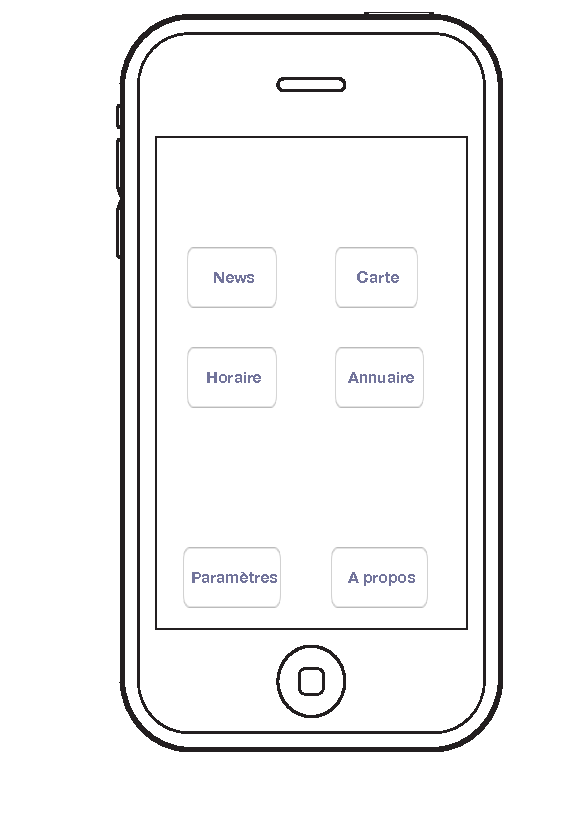
\includegraphics[width=0.3\textwidth]{../comon/figures/MainMenuIPhone.pdf}} 
					\subfigure[Navigation sur IPad]{\label{MainMenuIPad}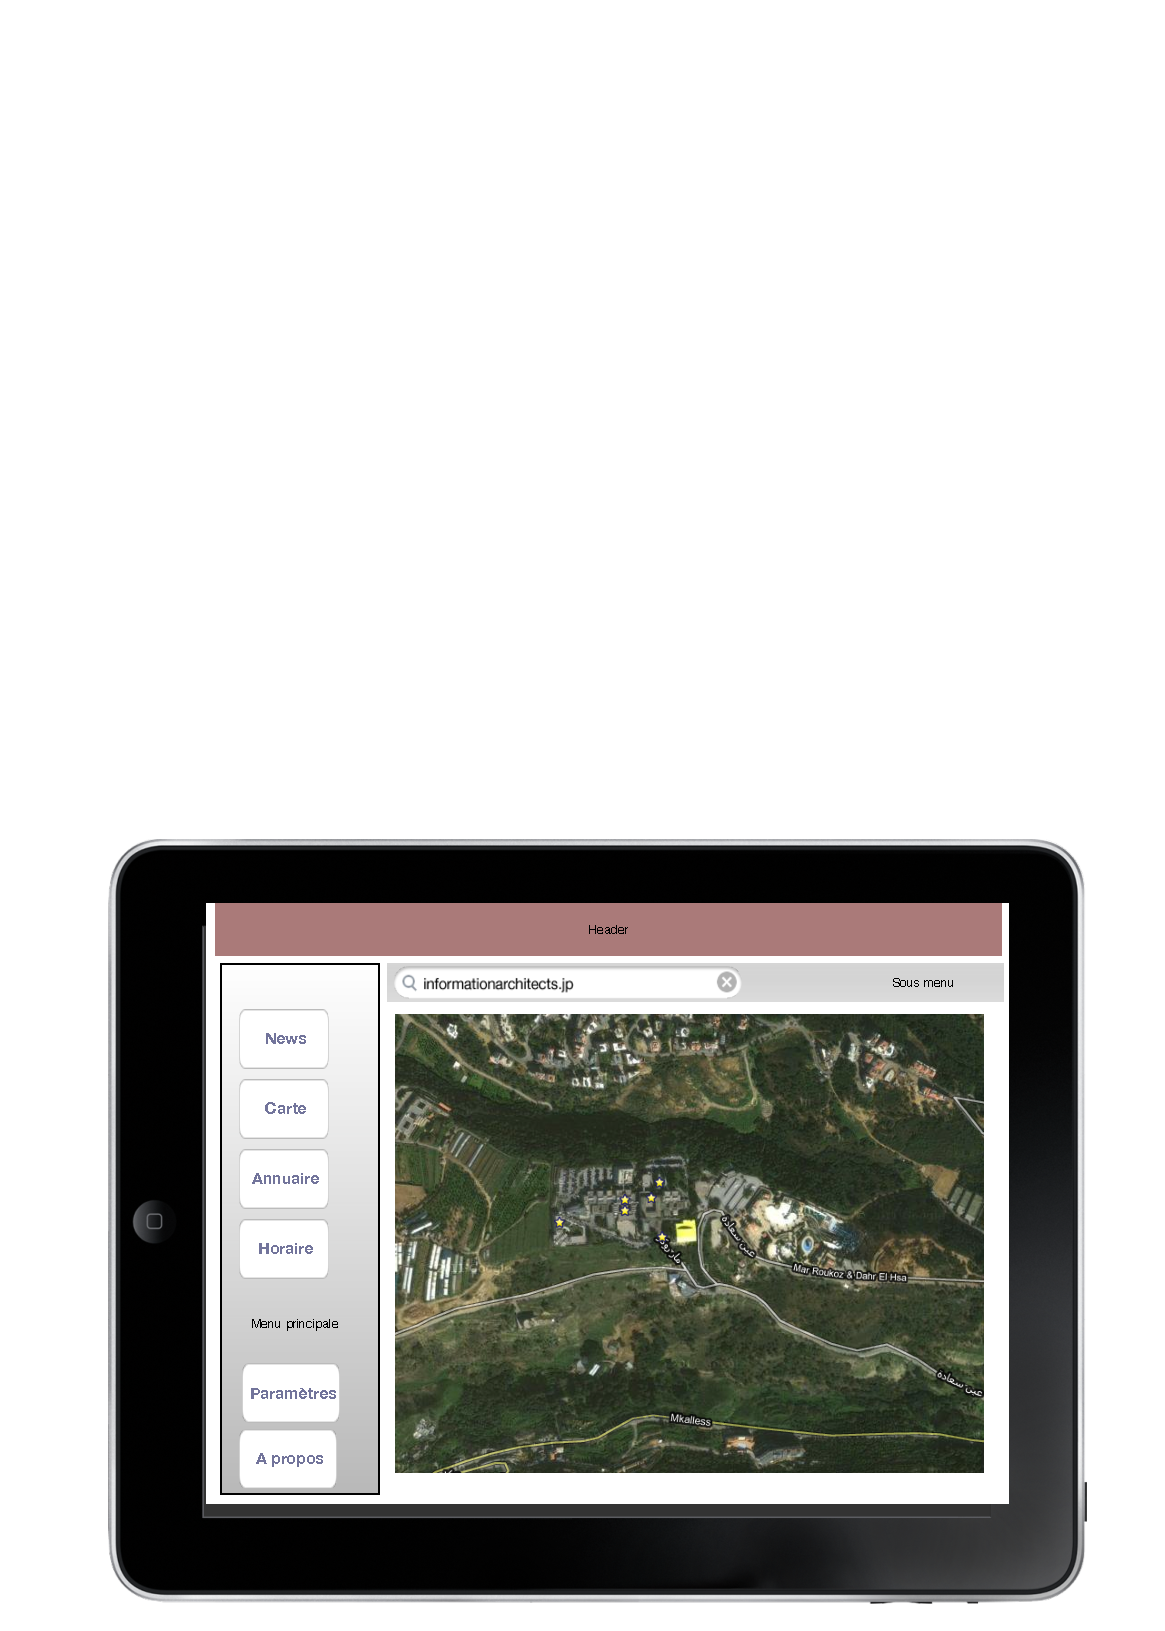
\includegraphics[width=0.6\textwidth]{../comon/figures/MainMenuIPad.pdf}} 
				\end{figure}
				
				
				
		\subsubsection{Paramétrer l'application}
			L'utilisateur doit pouvoir choisir les paramètres de l'application et les sauvegarder.\\[0.2cm]
			\begin{longtable}{|l|p{10cm}|}
				\hline \textbf{Nom du Use Case} & Paramétrage \\ 
				\hline \textbf{Ref} & UC\_1  \\ 
				\hline \textbf{Déclencheur} & L'utilisateur clique sur le bouton paramètre de la navigation\\
				\hline \textbf{Précondition} &  \\
				\hline \textbf{Scénario nominal} & 
				\begin{enumerate}
					\item Le système restaure les valeurs des paramètres depuis le fichier de configuration et les affiche.
					\item L'utilisateur choisit une option qu'il désire modifier.
					\item L'utilisateur modifie la valeur.
					\item \label{uc1Mod}L'utilisateur confirme qu'il a finit de modifier la valeur
					\item Le système sauvegarde la valeur.
				\end{enumerate}
				\\ 
				\hline \textbf{Enchaînements alternatifs} &  \\
				\hline \textbf{Status actuel} & Planifié:\CheckedBox , Implémenté:\CheckedBox , Testé: \CheckedBox , Validé: \CheckedBox \\
				\hline 
			\end{longtable} 
		\subsubsection*{Besoin graphique}
		\EPSFIGTEXTWIDTH{../comon/figures/WierframeIPhoneSettings.pdf}{Wireframe illustrant les modifications des paramètres sur l'iPhone}{WierframeIPhoneSettings}
		
		\EPSFIGTEXTWIDTH{../comon/figures/WierframeIPadSettings.pdf}{Wireframe illustrant les modifications des paramètres sur l'iPad}{WierframeIPadSettings}


		\subsubsection{Visualiser la carte}
					L'utilisateur doit pouvoir visualiser la carte du campus avec les différentes informations utiles pour se retrouver dans le campus.\\[0.2cm]
					\begin{longtable}{|l|p{10cm}|}
						\hline \textbf{Nom du Use Case} & Carte \\ 
						\hline \textbf{Ref} & UC\_3  \\ 
						\hline \textbf{Déclencheur} & L'utilisateur presse sur le bouton carte de l'application \\
						\hline \textbf{Précondition} &  \\
						\hline \textbf{Scénario nominal} & 
						\begin{enumerate}
							\item Le système affiche la carte de tous les campus ainsi que la position actuelle de l'utilisateur.
							\item Le système permet de choisir un campus pour en voir le détail.
							\item Le système affiche les bâtiments principaux du campus.
							\item Le système permet de naviguer, sélectionner des bâtiments ou une personne pour les afficher sur la carte.
						\end{enumerate}
						\\ 
						\hline \textbf{Enchaînements alternatifs} & \\
						\hline \textbf{Status actuel} & Planifié:\CheckedBox , Implémenté:\CheckedBox  , Testé: \CheckedBox  , Validé: \CheckedBox  \\
						\hline 
					\end{longtable} 
			\subsubsection*{Besoin graphique}
					\EPSFIGTEXTWIDTH{../comon/figures/MapIPhone.pdf}{Wireframe illustrant les fenêtres de l'affichage des cartes sur l'iPone}{MapIPhone}

					\EPSFIGTEXTWIDTH{../comon/figures/MapIPad.pdf}{Wireframe illustrant les fenêtres de l'affichage des cartes sur l'iPad}{MapIPad}
					Sur la Figure~\ref{MapIPad} on peut voir, que les menus des deux versions sont les mêmes mais sur l'iPad, au lieu d'ouvrir chaque élément du menu dans une nouvelle fenêtre, les éléments sont ajouté comme des ''Pop-up'' dans la page principale.

	\subsubsection{Afficher les nouvelles}
					L'utilisateur doit pouvoir visualiser les nouvelles du campus .\\[0.2cm]
					\begin{longtable}{|l|p{10cm}|}
						\hline \textbf{Nom du Use Case} & AfficherNews \\ 
						\hline \textbf{Ref} & UC\_4  \\ 
						\hline \textbf{Déclencheur} & L'utilisateur presse sur le bouton news de l'application \\
						\hline \textbf{Précondition} &  \\
						\hline \textbf{Scénario nominal} & 
						\begin{enumerate}
							\item Le système affiche les news du campus.
							\item L'utilisateur peut cliquer sur une news pour voir le détail de cette dernière.
							\item Depuis le détail de la news, l'utilisateur peut, à l'aide d'un bouton retour, revenir à l'aperçu de l'ensemble des news.
						\end{enumerate}
						\\ 
						\hline \textbf{Enchaînements alternatifs} & \\
						\hline \textbf{Status actuel} & Planifié:\CheckedBox , Implémenté:\CheckedBox  , Testé: \CheckedBox  , Validé: \CheckedBox  \\
						\hline 
					\end{longtable} 
			\subsubsection*{Besoin graphique}
					\EPSFIGTEXTWIDTH{../comon/figures/WierframeIPhoneNews.pdf}{Wireframe illustrant les fenêtres de l'affichage des news sur l'iPone}{WierframeIPhoneNews}

					\EPSFIGTEXTWIDTH{../comon/figures/WierframeIPadNews.pdf}{Wireframe illustrant les fenêtres de l'affichage des news sur l'iPad}{WierframeIPadNews}


			\subsubsection{Afficher l'annuaire}
					L'utilisateur doit pouvoir visualiser l'annuaire de l'USJ.\\[0.2cm]
					\begin{longtable}{|l|p{10cm}|}
						\hline \textbf{Nom du Use Case} & AfficherAnnuaire \\ 
						\hline \textbf{Ref} & UC\_5  \\ 
						\hline \textbf{Déclencheur} & L'utilisateur presse sur le bouton annuaire  de l'application \\
						\hline \textbf{Précondition} &  \\
						\hline \textbf{Scénario nominal} & 
						\begin{enumerate}
							\item Le système affiche la liste des possibilités de regroupement:
								\begin{enumerate}
									\item Par campus
									\item Par institution
									\item Services
								\end{enumerate}
							\item L'utilisateur choisit un regroupement qu'il veut
							\item L'utilisateur choisit le sous-groupe désiré.
							\item Le système cherche les données en cache si elles s'y trouvent sinon depuis les services web.
							\item Le système affiche la liste des personnes trouvées.
							\item L'utilisateur presse sur le bouton pour obtenir plus de détail d'une personne.
							\item Le système affiche le détail de la personne.
							\item Le système permet le démarrage d'appel sur un clique sur le numéro de téléphone ou l'envoi d'un e-mail suite à un clique sur l'adresse mail.
						\end{enumerate}
						\\ 
						\hline \textbf{Enchaînements alternatifs} & \\
						\hline \textbf{Status actuel} & Planifié:\CheckedBox , Implémenté:\CheckedBox  , Testé: \CheckedBox  , Validé: \CheckedBox  \\
						\hline 
					\end{longtable} 
			\subsubsection*{Besoin graphique}
					\EPSFIGTEXTWIDTH{../comon/figures/WierframeIPhoneDirectory.pdf}{Wireframe illustrant les fenêtres de l'affichage de l'annuaire sur l'iPone}{WierframeIPhoneDirectory}

					\EPSFIGTEXTWIDTH{../comon/figures/WierframeIPadDirectory.pdf}{Wireframe illustrant les fenêtres de l'affichage de l'annuaire sur l'iPad}{WierframeIPadDirectory}


			\subsubsection{Afficher l'horaire}
								Les utilisateurs de l'USJ  doivent pouvoir visualiser leurs horaires.\\[0.2cm]
								\begin{longtable}{|l|p{10cm}|}
									\hline \textbf{Nom du Use Case} & AfficherHoraire \\ 
									\hline \textbf{Ref} & UC\_6  \\ 
									\hline \textbf{Déclencheur} & L'utilisateur presse sur le bouton horaire de l'application \\
									\hline \textbf{Précondition} &  \\
									\hline \textbf{Scénario nominal} & 
									\begin{enumerate}
										\item Le système affiche un calendrier contenant le jour courant. 
										\item L'utilisateur peut naviguer facilement au jours suivants et précédents. 
										\item L'utilisateur peut, en cliquant sur un cours, afficher son emplacement.
									\end{enumerate}
									\\ 
									\hline \textbf{Enchaînements alternatifs} & \\
									\hline \textbf{Status actuel} & Planifié:\CheckedBox , Implémenté:\CheckedBox  , Testé: \CheckedBox  , Validé: \CheckedBox	  \\
									\hline 
								\end{longtable} 
						\subsubsection*{Besoin graphique}
								\EPSFIGTEXTWIDTH{../comon/figures/wireframeHorraireIPhone.pdf}{Wireframe illustrant les fenêtres de l'horaire sur l'iPone}{WierframeIPhoneNews}
			
								\EPSFIGTEXTWIDTH{../comon/figures/wireframeHorraireIPad.pdf}{Wireframe illustrant les fenêtres de l'horaire sur l'iPad}{WierframeIPadNews}
								

			\subsubsection{Afficher le résultat des examens}
								Les étudiants de l'USJ doivent pouvoir visualiser leurs résultats d'examen.\\[0.2cm]
								\begin{longtable}{|l|p{10cm}|}
									\hline \textbf{Nom du Use Case} & AfficherNoteExamen \\ 
									\hline \textbf{Ref} & UC\_7  \\ 
									\hline \textbf{Déclencheur} & L'utilisateur presse sur le bouton résultat d'examen de l'application \\
									\hline \textbf{Précondition} &  \\
									\hline \textbf{Scénario nominal} & 
									\begin{enumerate}
										\item Le système affiche la liste des examens et la note obtenue. 
									\end{enumerate}
									\\ 
									\hline \textbf{Enchaînements alternatifs} & 
										Commence au point 0 du scénario  nominal quand l'utilisateur n'est pas un étudiant.
									\begin{enumerate}
										\item Le système affiche un message d'erreur.
										\item Le système redirige l'utilisateur vers la fenêtre de paramétrage de l'application.
									\end{enumerate}\\
									\hline \textbf{Status actuel} & Planifié:\CheckedBox , Implémenté:\CheckedBox  , Testé: \CheckedBox  , Validé: \CheckedBox	  \\
									\hline 
								\end{longtable} 
						\subsubsection*{Besoin graphique}
								\EPSFIGSCALE[1.5]{../comon/figures/wireframeNoteIPhone.pdf}{Wireframe illustrant les fenêtres des résultats d'examen sur l'iPone}{WierframeIPhoneNews}
			
								\EPSFIGSCALE[1.5]{../comon/figures/wireframeNoteIPad.pdf}{Wireframe illustrant les fenêtres des résultats d'examen sur l'iPad}{WierframeIPadNews}
